% \begin{document}
\chapter{Problemi e Modelli}

\section{Problemi di ottimizzazione}

\dfn{Ricerca operativa}{
  La \textbf{ricerca operativa} è un ramo della matematica applicata che si occupa dello studio, della modellizzazione e della risoluzione dei cosiddetti \textit{problemi decisionali} complessi mediante strumenti matematici, algoritmici e computazionali, con l'obiettivo di ottimizzare processi e risorse
}

Per evitare qualsivoglia fraintendimento fornirò anche la definizione di \textbf{ottimizzazione Combinatoria}
\dfn{Ottimizzazione Combinatoria}{
  Si definisce \textbf{Ottimizzazione Combinatoria} una branca della Ricerca Operativa che nel modellare matematicamente e risolvere problemi complessi di natura discreta unisce tecniche di calcolo combinatorio alla teoria degli algoritmi e ai risultati teorici e metodologici della programmazione lineare
}

Pertanto ricerca operativa e ottimizzazione combinatoria sono due cose diverse, MA cito testualmente
\begin{quote}
  "Per tutti i nostri scopi ricerca operativa e ottimizzazione, sono sinonimi

  tuttavia non vedremo solo alcune tecniche di ottimizzazione combinatoria, ma anche altre tecniche che stanno nella ricerca operativa ma che trattano di valori non discreti"

  \hfill -- Ugo
\end{quote}

Adesso, sotterrato questo problema di carattere unicamente terminologico con cui io non posso fare a meno di strizzarmi il cervello perché c'ho l'autismo, possiamo tornare a parlare di ricerca operativa/ottimizzazione combinatoria (tanto so' sinonimi per noi)

I problemi di cui si occupa la ricerca operativa, quindi, riguardano situazioni in cui occorra massimizzare i ricavi o minimizzare i costi, in presenza di risorse limitate. Detto in termini più matematici, data una funzione \textbf{vincolata} l'obiettivo è trovare una soluzione ottimale che massimizzi o minimizzi tale funzione.

È pertanto vero, quindi, che questa disciplina ha forte contenuto economico

La ricerca operativa si inserisce all'interno del processo decisionale, il quale può essere suddiviso in diverse fasi
\begin{itemize}
\item \textbf{Individuazione problema}
  \item \textbf{Raccolta dati}
    \item \textbf{Costruzione modello}, ovvero la Traduzione del problema in un modello matematico che descriva il sistema e i vincoli in modo formale
      \item \textbf{Determinazione di piu' soluzioni}: applicazione di algoritmi e tecniche di ottimizzazione per individuare la soluzione migliore 
  \item \textbf{Analisi dei risultati}
\end{itemize}

La ricerca operativa, quindi, si occupa delle fasi 3 e 4 del processo, dato che sono le fasi che richiedono l’impiego di modelli matematici, algoritmi di ottimizzazione e strumenti computazionali. Adesso andiamo a definire per benino che cosa intendiamo per "modello" 

\dfn{modello}{
  un \textbf{modello} è una descrizione astratta e scritta in linguaggio matematico, della parte di realtà utile al processo decisionale
}
I modelli ci permettono di inquadrare i problemi in una determinata "cornice" che ci permette di determinare quale tipo di algoritmo risolutivo usare.

Esistono tre tipi di modelli:
\begin{itemize}
\item \textbf{Teoria dei giochi}: ricerca di un equilibrio fra le componenti coinvolte in un'interazione reciproca, spesso con obbiettivi contrastanti. (non ce ne occupiamo)
\item \textbf{Simulazione}: il problema viene studiato simulando la situazione senza studiarne la natura in modo analitico tramite generazione di istanze casuali. (anche questi modelli non ci interessano)
\item \textbf{Analitici}: dal problema si costruisce un modello matematico rigoroso (senza perdere informazione sul problema reale) e risolto mediante tecniche analitiche, senza ricorrere a simulazioni. La natura stessa dello spazio matematico in cui è inserito il problema è in grado di garantire la soluzione ottima. Questo tipo approccio è particolarmente vantaggioso in quanto assicura l’esattezza della soluzione supponendo che il modello sia formulato correttamente. 

È tuttavia richiesto un discreto livello di creatività
\end{itemize}

Definiamo, adesso, i problemi che andiamo a trattare

\dfn{Problema}{
  Definiamo \textbf{problema} una domanda, espressa in termini generali, la cui risposta dipende da \textit{parametri} e \textit{variabili}, sopratutto nei problemi analitici
}
Un problema $ \mathcal{P} $ è descritto tramite:
\begin{itemize}
  \item I suoi parametri e variabili
  \item Le caratteristiche che una soluzione deve avere
\end{itemize}

Quando fissiamo un'istanza di un problema, vengono fissati i parametri ma non le variabili, che sono le incognite che devono essere definite. Distinguiamo un problema dalla sua istanza per generalizzarlo. Si presti attenzione alla differenza tra parametri e variabili che molti si confondono

\ex{Problema con paramteri e variabili}{
  Sia $ \mathcal{P} $ il seguente problema
  \[
    ax^2+bx+c =0
  \]
  Dove $a,b$ e $c$ sono i suoi parametri e $x$ rappresenta le variabili, una possibile istanza di tale problema è:
  \[
    5x^2-6x+1=0
  \] 
}
Un modo comune per descrivere un problema è dare l'insieme di soluzioni ammissibili $ \mathbb{F}_{\mathcal{P}} \subseteq G $, dove $G$ è un sovrainsieme generico noto, di solito contenente la collezione di tutte le possibili configurazioni o decisioni che si possono prendere, dando dei vincoli che un generico $ g \in G $ deve soddisfare per far parte di $\mathbb{F}_{\mathcal{P}}$, avremo così che $G - \mathbb{F}_{\mathcal{P}}$ è l'insieme delle soluzioni non ammissibili 
\ex{}{
  Sia l'instanza di $\mathcal{P}$ definita precedentemente
  \[
    5x^s - 6x+1= 0
  \]
  si ha che 
  \[
    \begin{array}{l}
      \mathbb{G}= \mathbb{R}\\
      \mathbb{F}_{\mathcal{P}} = \{x\in \mathbb{R} | 5x^2-6x+1=0\}
    \end{array}
  \]
}
\subsection{2.1.1 Problemi di ottimizzazione}

Iniziamo con una definizione preliminare.

\dfn{Problema di ottimizzazione}{In matematica e in informatica, un problema di ottimizzazione è il problema di trovare la migliore soluzione fra tutte le soluzioni fattibili.}

Un problema di ottimizzazione $\mathcal{P}$ viene descritto:
\begin{itemize}
  \item Dando l’insieme $\mathbb{F}_\mathcal{P}$ delle soluzioni ammissibili
  \item Specificando una funzione obiettivo $c_\mathcal{P} : \mathbb{F}_\mathcal{P} \to \mathbb{R}$ che assegna ad ogni $g \in \mathbb{F}_\mathcal{P}$ un valore reale $c_\mathcal{P}(g)$, che rappresenta il costo o il beneficio.
\end{itemize}
Un problema (di ottimizzazione) di massimo $\mathcal{P}$ consiste nel determinare il valore
\[
Z_\mathcal{P} = \max \{ c_\mathcal{P}(g) \mid g \in \mathbb{F}_\mathcal{P} \},
\]
mentre un problema (di ottimizzazione) di minimo $\mathcal{P}$ consiste nel determinare il valore
\[
Z_\mathcal{P} = \min \{ c_\mathcal{P}(g) \mid g \in \mathbb{F}_\mathcal{P} \}.
\]
Ci si può trastullare con la definizione, infatti ad ogni problema di massimo $\mathcal{P}$ corrisponde un problema di minimo $\mathcal{P}'$ tale che $c_{\mathcal{P}'}(g) = -c_\mathcal{P}(g)$, ovvero:
\[
Z_\mathcal{P} = -\min \{ c_{\mathcal{P}'}(g) \mid g \in \mathbb{F}_\mathcal{P} = \mathbb{F}_{\mathcal{P}'} \}.
\]

\dfn{Valore ottimo e soluzione ottima}{Dato un problema di ottimizzazione $\mathcal{P}$, il valore $Z_\mathcal{P}$ definito in precedenza è detto valore ottimo, mentre il $g^* \in \mathbb{F}_\mathcal{P}$ tale che $Z_\mathcal{P} = c_\mathcal{P}(g^*)$ è detto soluzione ottima.}

Si può quindi constatare che la differenza reale tra i due è che il valore ottimo è inserito nel codominio della funzione obiettivo (cioè il mero valore reale “ottimizato”), mentre la soluzione ottima appartiene al dominio (ovvero è l’elemento in $\mathbb{F}_\mathcal{P}$ che ottimizza la funzione).

\ex{Esempio di problema di ottimizzazione}{Dati
\[
G = \mathbb{R}, \quad \mathbb{F}_\mathcal{P} = \{ x \in \mathbb{R} \mid 5x^2 - 6x + 1 = 0 \}, \quad c_\mathcal{P} : \mathbb{R} \to \mathbb{R} \text{ con } c_\mathcal{P}(g) = g^2,
\]
e si ponga
\[
Z_\mathcal{P} = \max \{ x^2 \mid x \in \mathbb{F}_\mathcal{P} \}.
\]
Innanzitutto, calcolo l’insieme delle soluzioni ammissibili (hold my soluzione parabolica):
\[
x = \frac{6 \pm \sqrt{(-6)^2 - 4\cdot5\cdot1}}{2\cdot5} = \frac{6 \pm \sqrt{36 - 20}}{10} = \frac{6 \pm \sqrt{16}}{10} = \frac{6 \pm 4}{10}.
\]
Quindi, le soluzioni sono:
\[
x_1 = \frac{6 + 4}{10} = 1 \quad \text{e} \quad x_2 = \frac{6 - 4}{10} = \frac{1}{5}.
\]
Pertanto, l’insieme delle soluzioni ammissibili è:
\[
\mathbb{F}_\mathcal{P} = \{ 1, \tfrac{1}{5} \}.
\]

Si procede poi nel calcolare la funzione obiettivo per ogni elemento:
\[
c_\mathcal{P}(1) = 1^2 = 1, \quad c_\mathcal{P}\left(\tfrac{1}{5}\right) = \left(\tfrac{1}{5}\right)^2 = \tfrac{1}{25}.
\]
Il massimo tra questi valori è:
\[
Z_\mathcal{P} = \max\{ 1, \tfrac{1}{25} \} = 1.
\]}

fin casi dei problemi di decisione

Si hanno quattro casi principali in cui sono inseriti i problemi di decisione:
\begin{itemize}
  \item \textbf{Problema vuoto:} non esistono soluzioni ammissibili, ovvero $\mathbb{F}_\mathcal{P} = \emptyset$, per cui l’ottimizzazione è impossibile e si assume che $Z_\mathcal{P} = \infty$.
  \item \textbf{Problema illimitato:} si ha quando non esiste un limite inferiore/superiore per i valori della funzione obiettivo tra le soluzioni ammissibili, ovvero quando $Z_\mathcal{P} = \pm\infty$. Ad esempio, nel caso del massimo, per ogni $x \in \mathbb{R}$ esiste un $g \in \mathbb{F}_\mathcal{P}$ con $c_\mathcal{P}(g) \ge x$, e quindi $Z_\mathcal{P} = +\infty$.
  \item \textbf{Valore ottimo finito ma non soluzione ottima finita:} un problema di ottimizzazione può presentare un valore ottimo finito, pur non ammettendo alcuna soluzione $g \in \mathbb{F}_\mathcal{P}$ tale che $c_\mathcal{P}(g)$ sia esattamente uguale a $Z_\mathcal{P}$. (Es.: nell’insieme $\{ x \mid x > 0 \}$, dove l’estremo inferiore è 0, ma non esiste una soluzione che raggiunga tale valore.)
  \item \textbf{Valore ottimo finito e soluzione ottima finita:} esiste almeno un $g \in \mathbb{F}_\mathcal{P}$ tale che $c_\mathcal{P}(g) = Z_\mathcal{P}$, ed esso è ottimo. Notare che possono esistere più soluzioni ottime, ma un solo valore ottimo.
\end{itemize}

\subsection{ Problemi di ottimizzazione e di decisione}

Verranno fornite due definizioni importanti:

\dfn{Problema di decisione}{Un problema di decisione consiste nel determinare una qualunque soluzione ammissibile $g \in \mathbb{F}_\mathcal{P}$.}

\dfn{Problema di certificato}{Il problema di certificato consiste nel verificare se, per un dato $g \in G$, risulti che $g \in \mathbb{F}_\mathcal{P}$.}

I problemi di decisione sono generalmente più semplici dei problemi di ottimizzazione, in quanto non richiedono la definizione di una funzione obiettivo $c_\mathcal{P}()$. Tuttavia, è possibile trasformarli in problemi di ottimizzazione fissando una funzione obiettivo triviale (ad esempio, costante), per cui tutte le soluzioni ammissibili risultano ottime.

In alternativa, possiamo considerare un problema decisionale $R$ definito da
\[
F_R = \{ g \in \mathbb{F}_\mathcal{P} \mid c_\mathcal{P}(g) = Z_\mathcal{P} \},
\]
oppure, per un dato $k \in \mathbb{R}$, il problema decisionale $R_k$ con
\[
F_{R_k} = \{ g \in \mathbb{F}_\mathcal{P} \mid c_\mathcal{P}(g) \le k \},
\]
nel caso in cui $\mathcal{P}$ sia un problema di minimo.

\subsection{Aspetto algoritmico}
\begin{itemize}
  \item Algoritmi esatti: e' un algoritmo ch epreso un'istanza di $ P $ ($ P $ e' un modello di un problema), fornisce in output una soluzione ottima $ g^* $ di $ P $ (se esiste). Spesso pero' i problemi sono troppo complessi ed e' impossibile costruire algoritmi efficenti.
  \item Algoritmi euristici: non ci danno garanzia sulla soluzione trovata (e' sicuramente ammissibile), ma un'approssimazione.
\end{itemize}

Come possiamo valutare la correttezza di una soluzione euristica? Possiamo misurare l'errore (assoluto o relativo) fra il valore ottimo euristico e quello esatto.

Gli algoritmi euristici vengono detti anche greedy.

\section{Modelli}
Al posto di dare un'algoritmo per ogni specifico problema, possiamo definire classi di problemi che possono essere risolti con lo stesso algoritmo.

\subsection{Programmazione Lineare}

Fornisco Innanzitutto la def. di problema di problema di Programmazione Lineare

\dfn{Problema di Programmazione Lineare}{
  Si definiscono \textbf{Problemi di programmazione lineare (PL)} tutti quei problemi di ottimizzazione in cui la funzione obbiettivo $c_{\mathcal{P}}$ è \textit{lineare} e i vincoli sono \textit{tutti espressi da disequazioni lineari} ed anche, eventualmente, equazioni lineari (quest'ultime possono mancare le prime no). 
  
  In particolare in un problema $\mathcal{P}$ di programmazione si ha:
  \begin{itemize}
    \item $\mathbb{G} = \mathbb{R}$, definendo poi un numero finito $n \in \mathbb{N}$ di variabili reali, che nella realtà rappresentano delle \textit{quantità}
    \[
      x = (x_1, \dots, x_n) \in \mathbb{R^N}
    \]
    \item Una \textit{funzione obiettivo} $c_{\mathcal{P}}$ definita $f : \mathbb{R}^n \to \mathbb{R}$ nella forma:
    \[
      f(x) = cx
    \]
    
    Dove $c$ è un vettore riga e $x$ è un vettore colonna. Si noti che $c$ non è una variabile, bensì un \textit{parametro} (definizione della funzione obiettivo)
    \item Un insieme di $m$ vincoli lineari, tutti in una delle forme seguenti:
    \[
      ax=b \quad ax\leq b \quad ax \geq b
    \]

    Dove $a\in \mathbb{R}^n$ e $b\in \mathbb{R}$
  \end{itemize}
}

$ f $ e' lineare. 
$ c_p $ e' l'insieme di vettori di numeri reali. $ \mathbb{G} = \mathbb{R}^n $. (definizione di $ G $)

È talvolta utile assumere che $x \in \mathbb{Z}^n$, ovvero che le soluzioni ammissibili siano vettori di numeri interi. In questo caso si parla di \textit{programmazione lineare intera}. Facendo così, stiamo restringendo il campo di ricerca (ed il dominio delle soluzioni possibili), ma si perdono alcune proprietà (geometriche) che in realtà possono rendere più difficile la ricerca della soluzione. 

Esiste inoltre la \textit{programmazione lineare mista} (PLM), dove si hanno variabili di natura mista (alcune variabili in $ \mathbb{R} $ ed alcune in $ \mathbb{Z} $)

Si noti questo diagramma riassuntivo:

\begin{center}
  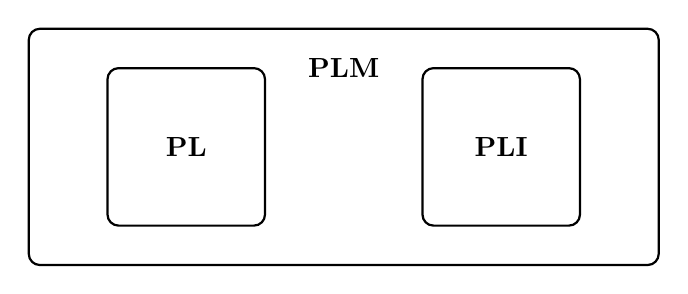
\begin{tikzpicture}
    
    \draw[thick, rounded corners] (-4, -1.5) rectangle (4, 1.5);
    
    \draw[thick, rounded corners] (-3, -1) rectangle (-1, 1);
    \node at (-2, 0) {\textbf{PL}};
    
    \draw[thick, rounded corners] (1, -1) rectangle (3, 1);
    \node at (2, 0) {\textbf{PLI}};
    
    \node at (0, 1) {\textbf{PLM}};
    
  \end{tikzpicture}
\end{center}
  
  


Un problema PL può sempre essere espresso nella seguente forma matriciale:
\[
  \max \{cx \mid Ax \leq b\}
\]
dove $ A \in \mathbb{R}^{m \times n} $ e $ b \in \mathbb{R}^m $. Grazie ad alcuni accorgimenti è possibile, inoltre, scrivere tutti i vincoli possibili di un problema di PL $\mathcal{P}$ in un'unico sistema di disequazioni lineari. Infatti:
\begin{itemize}
  \item Se \p è un problema di minimo, occorre considerare semplicemente la funzione $f (x) = (-c)x$
  \item Ogni vincolo $ax = b $diventa la coppia di vincoli $ax \leq b$ e $ax \geq b$
  \item Ogni vincolo $ax \geq b$ è equivalente a $(-a)x \leq (-b)$.
\end{itemize}

\subsection{Programmazione lineare intera}
Se nella $PL$ le variabili rappresentano quantità 
\begin{itemize}
\item Quantita'
\item Logiche: catturare valori booleani, quindi non scelte rispetto al "quanto" ma al "se", ovvero l'opportunita' di fare o meno una certa cosa
\end{itemize}

Una variabile $ x $ e' logica se:
\[
  x \in \mathbb{N} (o \mathbb{Z}) \quad 0\leq x \quad x \leq 1
\]

Tipico esempio sono le variabili che associano una certa risorsa a un task, o che venga usato un certo processo. Questo e' il bello dei problemi lineari. 

Esempi di problemi di ottimizzazione lineari:
\begin{itemize}
\item Lo Zaino
\item Albero di copertura minimo
\item Commesso viaggiatore
\end{itemize}

\subsection{Problema dello Zaino}
appunti scritti

Che tipo di relazioni logiche possiamo catturare con la programmazione lineare? TUTTEEEE con semplici vincoli lineari:
\begin{itemize}
  \item Negazione $ (y = \neg x) $: $ x = 1-y $
  \item Congiunzione $ (z = (x \land y)) $: 
    \[
    \begin{aligned}
      &z \leq x\\
      &z \leq y\\
      &z \geq x + y -1
    \end{aligned}
    \]
  \item Disgiunzione $ (z = (x \lor y)) $: 
    \[
    \begin{aligned}
      &z \geq x\\
      &z \geq y\\
      &z \leq x + y
    \end{aligned}
    \]
  \item Implicazione $ (z = (x \implies y)) $:
    \[
    \begin{aligned}
      &x+z \geq 1\\
      &z \geq y\\
      &x+z \leq 1 + y
    \end{aligned}
    \]
\end{itemize}

Questa cosa e' un'evidenza del fatto che il problema lineare di ottimizzazione e' in generale NP-hard :(. In poche parole e' perche' il problema di soddisfacibilita' di una formula logica e' nella classe NP-hard.

\section{Template per risolvere problemi}

\subsection{Vincoli di assegnamento}

Problemi che riguardano situazioni in qui dobbiamo assegnare "oggetti a luoghi". L'insieme $ N $ di oggetti possono essere automezzi, persone, ... mentre i luoghi $ V $ devono ricevere uno e solo un oggetto. Dobbiamo catturare il significato che l'i-esimo oggetto e' stato assegnato al j-esimo luogo.

Prendiamo le variabili logiche $ x_{ij} =  $

Vincoli di Semi-Assegnamento: ogni oggetto e' assegnato a un luogo, ma non ogni luogo riceve un oggetto
\[
  \sum_{j=1}^{m} x_{ij} = 1 \quad (1 \leq i \leq n)
\]

Insiemi ammissibili:

Vincoli di Assegnamento: ogni oggetto e' assegnato ad un luogo e ogni luogo ha un oggetto
\[
  \sum_{j=1}^{m} x_{ij} = 1 \quad (1 \leq i \leq n) \qquad \sum_{i=1}^{n} x_{ij} = 1 \quad (1 \leq j \leq m)
\]

Ordinamento
il luogo puo' anche essere visto come uno slot temporale, quindi imponiamo un certo pipeline

